\documentclass[a4paper 12pt]{article}
\usepackage[margin=1in]{geometry}
\usepackage{natbib}
\usepackage{epsfig}
\usepackage{amsmath}
\usepackage{amsfonts}
\usepackage{float}
\usepackage{rotating} 
\usepackage{caption}
\usepackage{subfig}
\usepackage{booktabs}
\usepackage{adjustbox}
\usepackage[table]{xcolor}
\usepackage{tabularx}
\usepackage{caption}
\usepackage{enumerate}
\usepackage{enumitem}
\captionsetup{font=footnotesize}
\newcommand{\ra}[1]{\renewcommand{\arraystretch}{#1}}
\textheight 9.0 in
\textwidth 6.5 in
\topmargin -0.5 in
\oddsidemargin 0.0in
\renewcommand{\topfraction}{1}
\renewcommand{\bottomfraction}{1}
\renewcommand{\textfraction}{0}
\renewcommand{\floatpagefraction}{0.90}
\definecolor{TableEven}{rgb}{0.8000,0.9216,0.9490}
\usepackage{makecell}
%\usepackage{fourier} 
\numberwithin{equation}{section}
\usepackage{array}
\usepackage{titlesec}
\usepackage{sectsty}
\sectionfont{\centering}
\setcounter{secnumdepth}{4}
\usepackage{natbib}
\usepackage{siunitx}
\usepackage[toc,page]{appendix}


\renewcommand{\baselinestretch} {2.0}
\makeatletter
\setcounter{page}{1}
\def\doublespace{\def\baselinestretch{1}\@normalsize}
\def\enddoublespace{}
\title{\bf 
}   
% \footnotemark}
\author{}
\date{}
\@addtoreset{equation}{section}
\renewcommand{\sp}{\vspace{0.2 in}}
\renewcommand{\theequation} {\arabic{section}.\arabic{equation}}
%\renewcommand{\thefigure}{\arabic{section}.\arabic{figure}}
\renewcommand{\thefootnote}{\fnsymbol{footnote}}
\newtheorem{theorem}{Theorem}
\newtheorem{lemma}{Lemma}[section]
\newtheorem{remark}{Remark}[section]
\newtheorem{corollary}{Corollary}[section]
\newtheorem{exam}{Example}[section]
\newtheorem{proposition}{Proposition}[section]

\newcommand{\Bigskip}{\vspace{0.3 in}}

\usepackage{xspace}
\newcommand{\m}{\textnormal{\sffamily m}\xspace}
\newcommand{\cm}{\textnormal{\sffamily cm}\xspace}
\newcommand{\g}{\textnormal{\sffamily g}\xspace}
\newcommand{\kg}{\textnormal{\sffamily kg}\xspace}


\makeatletter
\let\latex@xfloat=\@xfloat
\def\@xfloat #1[#2]{%
  \latex@xfloat #1[#2]%
  \def\baselinestretch{1}
  \@normalsize\normalsize
  \normalsize
}
\makeatother

\newcommand\longitude[1]{\directlua{ longitude ( \luastring{#1} ) }}


\usepackage{lineno}
\linenumbers

 
\begin{document}
\title{Variance Estimators of North Sea International Bottom Trawl Survey Indices}

\maketitle


\begin{abstract}

\end{abstract}
%Fisheries managers rely heavily on fish stock assessments to provide them with a foundation for their management decisions.\\

%A major conclusion of Walters and Ludwig is that estimates of numbers of spawners and recruits are (of little value unless the accuracy of the estimates is also assessed. There is a parallel principle in the statistical estimation of model param- eters: the statistical estimates are of little value unless they are accompanied by estimates of their accuracy. A similar prin-ciple applies to management decisions which are based (in part) upon parameter estimates: uncertainty about parameter values cannot be ignored in forn~ulating management policy. These principles are valid even if observations are made with perfect accuracy. However, large observation errors (which are present in most fisheries data) result in substantial uncer- tainty in parameter estimates. The parameter uncertainty fre- quently overwhelms effects of density dependence in the stock-recruitment relationship. 111 such situations. more information is required before a rational strategy can be deter- mined. Then the first task of the manager is to obtain such information. This will usually require purposeful manipu- lation of the number of spawners.  

%uncertainty about parameter values cannot be ignored in formulating management policy

%The parameters used in stock assessment are known to have uncertainties associated with the stock  \\
%Estimates of parameters relating to stock size are of little value their accuracy is not assessed.
%\citep{walters1981effects}

%The North Sea International Bottom Trawl Surveys (NS-IBTS) dataset, coordinated by the International Council for Exploration of the Sea (ICES) is one such survey which provide information on seasonal distribution of stocks and estimates of abundance indices and catch in numbers of fish per age-class without an assessment of the accuracy of these estimates.  As pointed out by  \citet{ludwig1981measurement} estimates of parameters relating to stock size are of little value unless they are accompanied by estimates of measurement error variance. Estimates of abundance indices from the NS-IBTS are based on data from multistage sampling \\
\clearpage
\section{\large INTRODUCTION}
Fish stock assessments are relied on heavily by fishery managers for making management decisions regarding catch quotas. The assessments, which utilize many parameters provide fundamental information about the status of the stock, for instance, whether the stock is increasing and support for increased levels of harvest should be given, or whether the stock is decreasing and stricter control on harvest should be implemented. Associated with the many parameters used in fish stock assessment is the uncertainty about their estimates, which cannot be ignored when formulating management policies \citep{walters1981effects, ludwig1981measurement}. This uncertainty can arise from many sources including natural variability, estimation procedures and lack of knowledge regarding the parameter \citep{ehrhardt1997role}. The North Sea International Bottom Trawl Surveys (NS-IBTS) data, coordinated by the ICES, provides information on seasonal distribution of stocks and estimates of abundance indices and catch in numbers of fish per age-class without an assessment of the accuracy of these estimates.  As pointed out by  \citet{ludwig1981measurement} estimates of parameters relating to stock size are of little value unless they are accompanied by estimates of measurement error variance. The NS-IBTS estimates of abundance indices are based on data from a complex multi-stage stratified cluster sampling approach,  and  it is essential to account for the sampling complexities so as to produce reliable estimation and analysis \citep{lehtonen2004practical}. If the sampling complexities is ignored, the effect on the variance  of the parameters could be substantial, in  particular the variance could be greatly inflated  due to the clustering effect, which involves intra-cluster correlation of the variables \citep{lehtonen2004practical, aanes2015efficient}. 

 \begin{itemize}
 \item objectives of paper (including species of interest)
 \item indices and current estimators
 \item structure of paper
 \end{itemize}


 %and acocuntign for the sampling complexities is essential for reliable estimation and analysis \citep{lehtonen2004practical} \\
%For abundance at age composition an ALK approch is used....define ALK, which ALK procedure and the disadvantages (The second evaluation undertaken in
%this work is to assess the impact of borrowing ALKs for imputation.
%This practice is common in analysis of both fishery independent
%and fishery-dependent monitoring data, although
%the resulting impacts in terms of bias and overall accuracy is not
%well established.) of this procedure. What procedure we propose and the method of variance estimation is used (Variances are estimated nonparametrically using bootstrapping methods.)\\
%\indent The North Sea International Bottom Trawl Surveys uses a multistage \\
%
%
%In this paper we provide estimates of abundance at age and uncertainties for the NS-IBTS focusing on two species: \emph{Gadus morhua} (cod) and \emph{Pollachius virens} (saithe). The uncertainty is determined using non-parametric bootstrap \\
%
% \begin{itemize}
% \item objectives of paper (including species of interest)
% \item indices and current estimators
% \item structure of paper
% \end{itemize}

\subsection{History of the North Sea Internation Bottom Trawl Surveys}
\indent The North Sea International Bottom Trawl Surveys (NS-IBTS) was formed in 1991, which is a combination of the International Young Herring Survey (IYHS) and eight national surveys in the North Sea, Skagerrak and Kattegat areas. These surveys began in the 1960's, and the 1970's and 1980's, respectively. The IYHS was developed with the aim of obtaining annual recruitment indices for the combined North Sea herring \emph{Clupea harengus} stock (ICES 2012), but yielded valuable information on other fish species such as cod \emph{Gadus morhua} and haddock \emph{Melanogrammus aeglefinus}.\\
\indent The NS-IBTS began with quarterly surveys providing information on seasonal distribution of stocks sampled, hydrography and the environment, which allow changes in fish stock to be monitored and abundance of all fish species  (Table \ref{fishspecies}) to be determined. These quarterly surveys, however became difficult to sustain as countries experienced budget cuts making it impossible to maintain high levels of research vessel effort. As such, in 1997 countries carried out a survey only twice a year; a first quarter survey (January-February) and a third quarter survey (August-September). Table \ref{fishspecies} gives the scientific names (common names in parentheses) of the target species that are sampled during the quarterly North Sea International Bottom Trawl Surveys. The common names of the species in parentheses will be used in the rest of paper.\\

% spring and autumn of 1960 and 1961 with the aim of obtaining annual recruitment indices for the combined North Sea herring \emph{Clupea harengus} stock (ICES 2012), while the national surveys were developed in 1970's and 1980's.\\
%\indent The NS-IBTS began with quarterly surveys providing information on seasonal distribution of stocks sampled, which is necessary for monitoring changes in stock and determining abundance of all fish species (Table \ref{fishspecies}), and information on hydrography and the environment. However, these quarterly surveys became difficult to sustain as countries experienced budget cuts making it impossible to maintain high levels of research vessel effort, and in 1997 countries carried out a survey only twice a year; a first quarter survey (January-February) and a third quarter survey (August-September).\\

%\clearpage
\begin{table}[h!]
\centering
\setlength\tabcolsep{1.5pt} 
\captionsetup{font=small, width = 8.5cm}{
\caption{Species fished in IBTS 1991-2017.}\label{fishspecies}}
\begin{tabular}{cccccccccc}
\hline \\[0.1ex]
\multicolumn{2}{c}{} \\[0.1ex]
Standard Pelagic               & Standard Roundfish & By-Catch Gadoid       \\[1.5ex]
%\cmidrule(lr{0.5em}){1-1} \cmidrule(lr{0.5em}){2-2}\cmidrule(lr{0.5em}){3-3} \\ [0.1ex]
\hline \\[0.1ex]
 Clupea harengus (Herring) &  Gadus morhua (Cod)  & Pollachius (Pollock)      \\[1.5ex]
 Sprattus sprattus (Sprat)   & Melanogrammus aeglefinus (Haddock) & Trisopterus luscus (Pouting) \\[1.5ex]
 Scomber scombrus (Mackerel) & Trisopterus esmarkii (Norway Pout ) & Trisopterus minutus (Poor Cod) \\[1.5ex]
 & Pollachius virens (Saithe)  & Micromesistius poutassou (Blue Whiting)   \\[1.5ex]
& Merlangius merlangus (Whiting)  & Lysing (Hake)  \\[1.5ex]
& &  Molva molva (Ling) \\[1.5ex]
& &   Brosme brosme (Tusk) \\[0.5ex]
\hline
\end{tabular}
\end{table}

%\subsection{Survey Vessels, Timing and Geographic Coverage}
\indent Research vessels from seven (7) nations in the first quarter (Q1) and six (6) nations in the third quarter (Q3) are used for conducting surveys on all finfish species in the North Sea during January-February and July-August, respectively, in 1997-2017 (Table \ref{countries}). The sampling frame is defined by the ICES index or roundfish areas (RFA) as shown in Figure \ref{icesroufismap}, which we refer to as superstrata \citep{nottestad2015quantifying, fuller2011sampling}. These  roundfish areas were substratified into small strata defined by non-overlapping statistical rectangles of roughly $30 \times 30$ nautical miles ($1^{o} \  \mathrm{Longitude} \ \times  \  0.5^{o} \ \mathrm{Latitude}$), and were convenient to use for NS-IBTS as they were already being used for fisheries management purposes. Most statistical rectangles contain a number of possible tows that are deemed free of obstructions, and vessels are free to choose any position in the rectangles as long as the hauls are separated by at least 10 nautical miles within and between rectangles. However, to increase the randomisation of sampling, sampling locations are proposed in advance. These are based on a random selection on a random selection of valid tows with start and end position executed in the period 2000-2017. In some rectangles, sampling may be further stratified due to significant changes in seabed depth which may, in turn, cause variations in the fish population. In particular, the NS-IBTS herring, saithe and sprat data are weighted by depth strata in the statistical rectangle (Table \ref{weightings11}). It is also a requirement that countries avoid clustering their stations between adjacent rectangles in order to reduce positive serial correlation, and thereby maximize survey precision. \\
\indent The latest major reallocation of rectangles occurred in 1991, but since then the survey has tried to keep at least one vessel in every subarea in which it had fished in the most recent years. Each rectangle is typically sampled twice by two different countries, so that at least two hauls are taken per rectangle (Figure \ref{ibtsq1}), but intensified sampling is carried out in some rectangles in the Eastern English Channel, Southern North Sea and Central north Sea: at least 3 hauls per rectangle are taken in statistical rectangles  31F1, 31F2, 32F1, 33F4, 34F2, 34F3, 34F4, 35F3, 35F4; while six or more hauls per rectangle are taken in statistical rectangles  30F1, 32F2, 32F3, 33F2, 33F3 (ICES 1999).  The Skagerrak and Kattegat is fished solely by Sweden, who sample more than once in every rectangle while the west of Shetland (in Q1 and Q3) and inshore areas (Q3) is fished solely by Scotland. The edge of the Norwegian Trench is fished solely by Norway, but inshore areas near Denmark is fished by Denmark. The southern North Sea is fished by Denmark, Germany and England. France, typically, is the only country that surveys the western English Channel. Areas are surveyed by a single country because of the large proportion of untrawalable area (and subsequent gear damage issues experienced by other nations)  for efficient logistical purposes.\\
\indent In principle, the trawl tow locations are selected using a  semi-random approach with at least two primary sampling units (PSU) per stratum, where PSUs are standardized {\bf swept-area trawl hauls}. All countries, except England (in Q3) and Norway (in Q1 and Q3) randomly select hauling positions from a list of ``clear" (and in many circumstances previously visited) haul positions. The same haul positions are used by Norway and England every year. In the unusual event that no ``clear" tow exists the cruise leader, who select the haul positions, may select to undertake a ``blind" tow on unknown ground after checking the proposed trawl track for hazardous seadbed obstructions with acoustic methods. \\

%\clearpage 

\begin{table}[h!]
\centering
\captionsetup{font=small, width = 15.5cm}{
\caption{Survey country, vessel name, and period research vessels participating in first quarter (Q1) and third quarter (Q3) during 1997-2017.}\label{countries}}
\begin{tabular}{cccccccc}
\hline \\[0.1ex]
  & \multicolumn{2}{c}{\bf First Quarter (Q1)} & \multicolumn{2}{c}{\bf Third Quarter (Q3)}\\[1.5ex]
{\bf Country }  & Vessel name & Period    & Vessel name & Period  \\[0.5ex]
%\cmidrule(lr{0.5em}){2-3}  \cmidrule(lr{0.5em}){4-5} \\ [0.1ex]
\hline \\[0.5ex]
%\cmidrule(lr{0.5em}){1-1} \cmidrule(lr{0.8em}){2-2} \cmidrule(lr{0.5em}){3-3} \cmidrule(lr{0.5em}){4-4} \cmidrule(lr{0.8em}){5-5} \cmidrule(lr{0.5em}){6-6} \\ [0.1ex]
Denmark  &   Dana   &   January-February  & Dana & July-August    \\[1ex]
France  & Thalassa II & January-February & - & -   \\[1ex]
Germany   &  Walther  Herwig III & January-February   &   Walther  Herwig III & July-August \\[1ex]
Netherlands &  Tridens 2 &  January-February   & - & -     \\[1ex]
Norway  &   G.O. Sars  & January-February &    Johan Hjort  & July   \\[1ex]
UK England &- & -&  Endeavour &  August-September  \\[1ex]
UK Scotland   &  Scotia III &  January-February & Scotia III &  July-August \\[1ex]
Sweden  &  Dana &  January-February  &  Dana &  August                  \\[0.5ex]
\hline
\end{tabular}
\end{table}

%
%\begin{table}[h!]
%\centering
%\setlength\tabcolsep{1.5pt} 
%\captionsetup{font=small, width = 8.5cm}{
%\caption{Statistical rectangles with intensified sampling.}\label{rectangles}}
%\begin{tabular}{cccccccccccccccccc}
%\hline \\[0.1ex]
%\multicolumn{2}{c}{} \\[0.1ex]
%Trawl hauls & \multicolumn{9}{c}{Statistical Rectangles}       \\[1.5ex]
%%\cmidrule(lr{0.5em}){1-1} \cmidrule(lr{0.5em}){2-2}\cmidrule(lr{0.5em}){3-3} \\ [0.1ex]
%\hline \\[0.1ex]
% $ \geq 3$ &  31F1 & 31F2 & 32F1 & 33F4 & 34F2 & 34F3 & 34F4 & 35F3 & 35F4      \\[1.5ex]
% $ \geq 6$ &  30F1 & 32F2 & 32F3 & 33F2 & 33F3      \\[1.5ex]
%\hline
%\end{tabular}
%\end{table}


%\begin{figure}[h!]
%  \centering
% {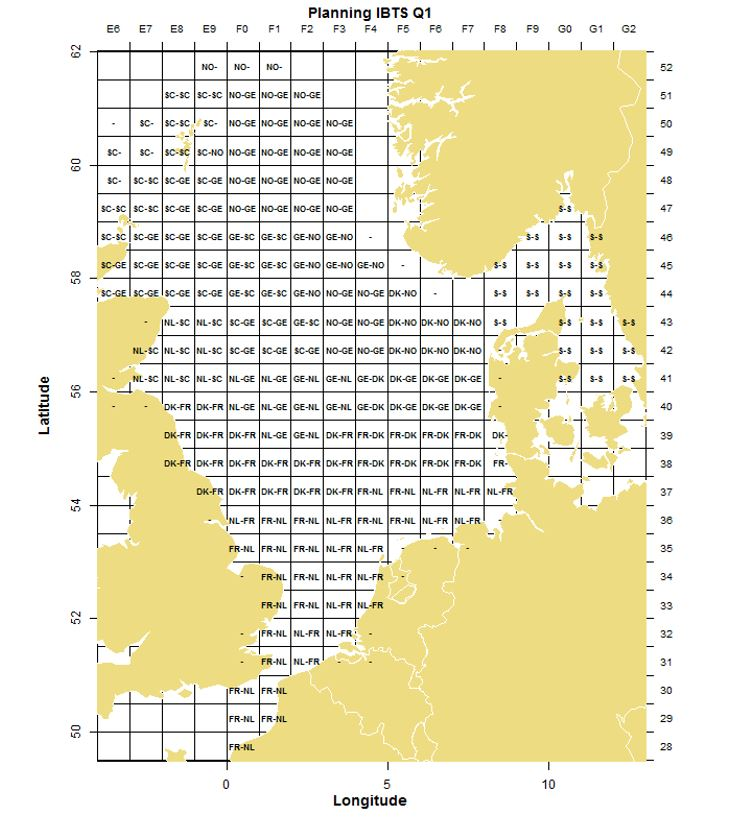
\includegraphics[width=18.5cm]{IBTSQ1.jpg}}   
% \captionsetup{font= footnotesize, width=15cm}{
% \caption{Spatial distribution of the ICES-rectangles in the IBTS Q1 over the participating countries. SC = Scotland, GE = Germany, NO = Norway, DK = Denmark, FR = France, NL = The Netherlands, S = Sweden (ICES 2016). }\label{ibtsq1}}
%\end{figure}
%
%
%
%\begin{figure}[h!]
%  \centering
% {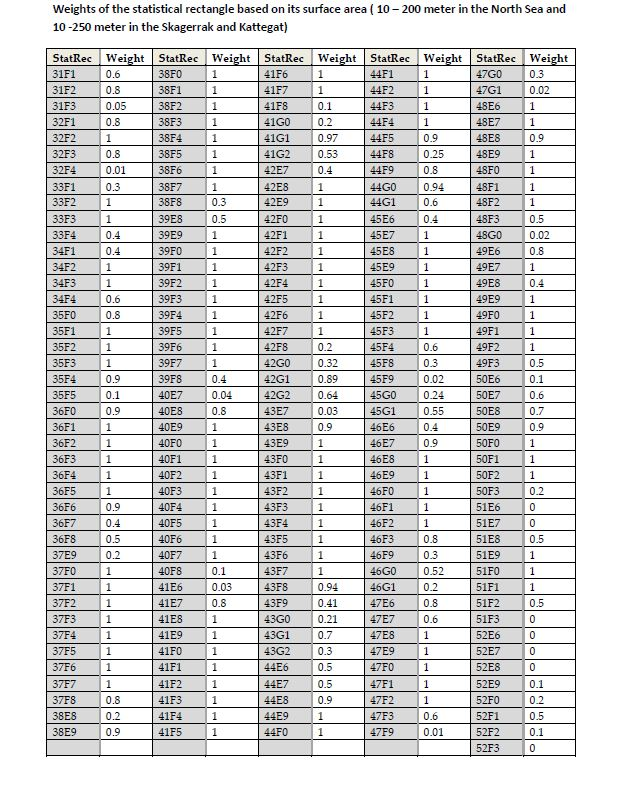
\includegraphics[width=17.5cm]{recWeightings.jpg}}   
% \captionsetup{font= footnotesize, width=15cm}{
% \caption{}\label{weightings11}}
%\end{figure}

%\clearpage
\subsection{Trawl Sampling and Protocols}
\label{trawlproto}
The mulitpurpose chalut {\`a} Grande Ouverture Verticale (GOV) trawl (ICES 2012) is the recommended standard gear of the IBTS and has been used on all participating vessels since 1992, while different pelagic and bottom trawls suitable for fishing finfish species were used before 1992. Since 1977, sampling of pelagic larvae during the International Bottom Trawl Survey in Q1 is also conducted using a  standard Midwater Ring Net, commonly known as MIK. Standardized trawling protocols were adopted with a towing speed of 4 knots but depending on vessel performance, tide and weather conditions the average towing speed can be at minimum 3.5 and maximum 4.5 knots. GOV with standard groundrope with rubber discs (groundgear A) for normal bottom conditions has been used throughout the survey area by all nations, except Scotland who since 1985 have used a hard ground gear for rough ground (groundgear B) on all stations north of   $52^\circ  \ 30''$ North  (ICES 2012). During the tow it is imperative that the net geometry of the gear is within the acceptable limits for the depth of water (Figure \ref{fig:test}). The trawls are towed in waters at a maximum depth of 200$\m$ in the North Sea and 250$\m$ in {\bf Division IIIa} with help of an ``Exocet"  kite and five floats attached to this kite. Rigging and trawl operation are described in (ICES 2012). The catching efficiency of the gear is assumed to be identical for every vessel. The tow duration was standardized to 30 minutes in {\bf 1978-2014} for all nations, except Scotland who maintained the tow duration of 60 minutes until 1998 (ICES 2015).  \\
\indent  In the third quarter (Q3) of 2015, an experiment on tow duration of NS-IBTS hauls was conducted in the North Sea to investigate the effect on the composition of catches, and which continued into the first quarter of 2016 (ICES 2015). In this paper we have not consider the NS-IBTS dataset for these periods.\\
\indent Trawling is done during the day by all participating vessels from 2000-2017 while countries who did not participate in the sampling of herring larvae in Q1 trawled at night before 2000. Daylight hours are considered 15 minutes before sunrise to 15 minutes  after sunset. After each trawl the total catch of the different species is weighed on board and biological parameters such as length for all fish species caught (to 0.1$\cm$ below for shellfish, to 0.5$\cm$ below for herring and sprat and to 1$\cm$ below for all other species) are collected. Where the numbers of individuals are too large for all of them  to be measured to obtain the length distribution, a representative subsample of 75 fish is selected. If a representative subsample cannot be selected further sorting of the species into two or more size grades or categories is necessary (ICES 2015). Otoliths are collected on board from a small fraction of all the target species from all RFA (Figure \ref{icesroufismap}) to retrieve age reading. However, from 2013 Norway has been sampling one otolith per length class from each trawl haul (to 0.1$\cm$ below for shellfish, to 0.5$\cm$ below for herring and sprat and to 1$\cm$ below for all other species).   \\ 
%Studies conducted by \citet{godo1990effect} and \citet{walsh1991diel} \citet{ehrich2001influence}
%Though the reduced time allows more hauls to be conducted during the survey time, and does not have a significant affect  on the length composition of catches, mean lengths of fish and catch per unit effort (God$ø$ et al. 1990, Walsh, 1991), Ehrich and Stransky (2001) found that the reduced time resulted in a slight decrease in the number of observed species but this was comparable with the reduced mean number of observed species from subsampling of very large hauls.\\

\clearpage
\begin{table}[h!]
\centering
\caption{Minimum sampling levels of otoliths by species for RFA.}
\label{otolithsTable}
\begin{tabularx}{\linewidth}{r l X}
\toprule 
 Species   	&  & Number of otoliths per length class in a RFA    \\[0.7ex]
\midrule \\[0.5ex]
 herring    	&  & $8$  otolihts per $\frac{1}{2}$ cm group \\[0.8ex]
sprat       &  & $16$  otolihts per $\frac{1}{2}$ cm group $8.0 -11.0$ cm\\[0.8ex]
            &  & $12$  otolihts per $\frac{1}{2}$ cm group $\geq 11.0$ cm\\[0.8ex]
mackerel    &  & $8$  otolihts per $\frac{1}{2}$ cm group \\[0.8ex]
cod       	&  & $8$  otolihts per $1$ cm group \\[0.8ex]
haddock   	&  & $8$  otolihts per $1$ cm group \\[0.8ex]
whiting    	&  & $8$  otolihts per $1$ cm group \\[0.8ex]
Norway pout &  & $8$  otolihts per $1$ cm group \\[0.8ex]
saithe      &  & $8$  otolihts per $1$ cm group \\[2ex] 
All target species    &  & from 2013 Norway has been sampling one otolith per length class from \\[0.7ex] 
&& each trawl haul (to 0.1$\cm$ below for shellfish, to 0.5$\cm$ below for herring and sprat and to 1$\cm$ below for all other species).\\[0.7ex] 
\bottomrule         
\end{tabularx}
\end{table}



\section{\large METHODS}
\label{methods}
The estimators used for the NS-IBTS data are haul time-based for computing catch per unit effort (cpue) indices. The indices are computed per roundfish area (superstrata), which are specific for each species. Indices are computed as mean per stratum (statistical rectangle) and then as mean of the strata  over the superstrata. The NS-IBTS data is registered as follows: 1) data calculated as catch in  numbers per hour trawled (denoted as C type), 2) data by haul (denoted as R type), and 3) sub-sampled data (denoted as S type). In this paper we account for the uncertainty in abundance at age in the North Sea. {\bf Two estimators based on ALK are considered to determine which estimator provides the most accurate estimates of precision given that the data are collected using a hierarchical design. The first is an ALK which is an aggregation of individual samples from a trawl haul combined over the round fish area (RFA), and which is the approach outlined by DATRAS}. The uncertainty in abundance at age is estimated using a \emph{simple nonparametric bootstrap} approach (Section \ref{simpleboot}) proposed by DATRAS, but which have not been implemented. This ALK approach does not account for haul to haul variation in age and length within the round fish area. The second is an ALK ........and we propose a \emph{stratified noparametric bootstrap} approach (Section \ref{stratboot})  \\

\begin{itemize}
\item ALK estimator - how is it tested?
\item Borrowing closest neighbour ALK for imputation? 
\item how efficiency of estimator is tested?
\item compare methods of variance estimation - nonparameteric bootstrap methods (simple, stratified, hierarchical?)
\end{itemize}


\subsection{Imputation for missing age samples}
Catches of the target species are sampled (or subsampled with a size of 75 if the catches are too large) for length, and otoliths are typically collected from a subsample of the individuals sampled for length in the RFA,  or for all trawl haul as in the case of Norway for determining age of the fish (see Table \ref{otolithsTable}). 


\begin{itemize}
\item Datras ALK approach (imputation approach) - does not account for variation in age-length groups within trawl hauls as length samples are trawl dependent - assume age-length groups are the same across hauls  
\item {\bf what is the ALK approach taken for the stratified bootstrap sampling method?}
\item ALk for each trawl haul (imputation approach) - considers haul to haul variaiton in age-lenght groups (explains the variance, improve estimation precision)

\item {\bf what is the estimator for age composition in the whole North Sea? - is it the average of $\mathrm{mCPUE}_{p,a} =  \sum\limits_{l \in L} \mathrm{mCPUE}_{p,a,l}$ in the 10 RFA? and how is the variance computed?}
\end{itemize}


\subsection{Estimators of length composition of fish}
\label{estimatorsoflength}
An estimator for the catch in numbers of fish per unit effort for a target species   per haul $h$ in length class $l$ by quarter, year, and stratum $s$ is expressed as the sum of the product of the number of fish in length class $l$ in a subsample $u$ and subfactor ($f_{u}$), multiplied by the trawling effort

\begin{equation}
\mathrm{CPUE}_{h,l} = \displaystyle \left(\sum\limits_{u \in U_{h}} n_{u,l}f_{u} \right) \times \frac{60}{d_{h}}
\label{cpuelength}
\end{equation}

\noindent where $n_{u} $, $f_{u}$ and $d_{h}$ are defined in Table \ref{symbols}. An estimator for the mean catch per unit effort for length class $l$ over hauls $H_{s}$ in stratum $s$  can be expressed as 

\begin{equation}
\mathrm{mCPUE}_{s,l} = \displaystyle\sum\limits_{h \in H_{s}} \frac{\mathrm{CPUE}_{h,l}}{|H_{s}|}.
\label{mcpuelength}
\end{equation}
\noindent where $|H_{s}|$ is the number of hauls in $s$. Similarly, an estimator for the mean catch per unit for length class $l$ in superstratum $p$ can be expressed as

\begin{equation}
\mathrm{mCPUE}_{p,l} = \sum\limits_{s \in S_{p}} \frac{\mathrm{CPUE}_{s,l}}{|S_{p}|}.
\label{mcpuelengthrfa}
\end{equation}

where $|S_{p}|$ is the number of strata in $p$ (Table \ref{symbols}). ICES (2006) provides a nonparametric bootstrap variance estimator for equation (\ref{mcpuelengthrfa}), which we describe in Section \ref{simpleboot}. \\

%\clearpage
\begin{table}[h!]
\centering
\caption{List of symbols and parameters used.}
\label{symbols}
\begin{tabularx}{\linewidth}{r l X}
\toprule 
Symbol   	&  & Definition                  \\[0.7ex]
\midrule
$L$        	&  & The set of length classes    \\[0.7ex]
$A$        	&  & The set of age groups       \\[0.7ex]
$|A|$      	&  & The number of age groups    \\[0.7ex]
$P$        	&  & The set of superstrata      \\[0.7ex]
$|P|$       &  & The number of superstrata   \\[0.7ex]
$S_{p}$     &  & The set of strata in superstrata $p$  \\[0.7ex]
$|S_{p}|$   &  & The number of strata in $p$  \\[0.7ex]
$H_{s}$     &  & The set of hauls in strata $s$  \\[0.7ex]
$|H_{s}|$   &  & The number of hauls in $s$  \\[0.7ex]
$U_{h}$     &  & The set of subsamples from haul $h$  \\[0.7ex]
$|f_{u}|$   &  & The subfactor for the subsample $u$. The subfactor $|f_{u}|$ is always 1 for C-type data  \\[0.7ex]
$n_{u,l}$   &  & The number of fish of target species in length class $l$ in subsample $u$  \\[0.7ex]
$d_{h}$   &  & The duration (minutes) for haul $h$  \\[0.7ex]
ALK  & & The age-length key for the target species is .......\\
\bottomrule         
\end{tabularx}
\end{table}

%
%\begin{table}[h!]
%\centering
%\caption{Summary of estimators.}
%\label{estimators}
%\begin{tabularx}{\linewidth}{r l l l  X}
%\toprule 
%Estimator   	&  & Definition && Comment                  \\[0.7ex]
%\midrule
%$\mathrm{CPUE}_{h,l}$   &  & \thead{Catch in numbers per hour trawled (CPUE)\\  of target species in length class $l$ in haul $h$}  \\[0.7ex]
%
%$\mathrm{CPUE}_{h,l}$   &  & \thead{Catch in numbers per hour trawled (CPUE)\\  of target species in length class $l$ in haul $h$}  \\[0.7ex]
%
%$\mathrm{CPUE}_{h,l}$   &  & \thead{Catch in numbers per hour trawled (CPUE)\\  of target species in length class $l$ in haul $h$}  \\[0.7ex]
%\bottomrule         
%\end{tabularx}
%\end{table}





\subsection{Estimators of age composition of fish}
\label{agecom}

An estimator of the catch per unit effort for length class $l$ and age group $a$ in haul $h$ is expressed as the ratio

\begin{equation}
\mathrm{CPUE}_{h,a,l} =  \displaystyle \frac{\mathrm{CPUE}_{h,l} \times \mathrm{ALK}_{a,l}}{\displaystyle \sum\limits_{a \in A} \mathrm{ALK_{a,l}}}.
\label{cpueage}
\end{equation}

\noindent where $\mathrm{ALK}_{a,l} $ is the number of fish at age $a$ in length class $l$, and $\mathrm{CPUE}_{h,l} $ is the catch per unit effort for length class $l$ in haul $h$ in stratum $s$ defined in equation (\ref{cpuelength}). The mean catch per unit effort for length class $l$ over hauls $H_{s}$ in stratum $s$ by year and quarter is therefore expressed as 

 \begin{equation}
\mathrm{mCPUE}_{s,a,l} = \sum\limits_{h \in H_{s}} \frac{\mathrm{CPUE}_{h,a,l}}{|H_{s}|}.
\label{mcpueage}
\end{equation} 

An estimator of the mean catch per unit effort for length class $l$ in superstratum $p$ is expressed as


\begin{equation}
\mathrm{mCPUE}_{p,a,l} =  \sum\limits_{s \in S_{p}} \frac{\mathrm{mCPUE}_{s,a,l}}{|S_{p}|}.
\label{mcpueagerfa}
\end{equation}

An index of abundance by age is computed by taking the sum of the length classes for a given age within the round fish area. This is the mean catch per unit effort for age $a$ in superstratum $p$, which is expressed as

\begin{equation}
\mathrm{mCPUE}_{p,a} =  \sum\limits_{l \in L} \mathrm{mCPUE}_{p,a,l}.
\label{ageIndex}
\end{equation}



\subsection{Variance estimation}
\label{bootall}
The variance of the estimated CPUEs are calculated with bootstrap procedures. In this section we elaborate the bootstrap procedures used in this paper. We have implemented two procedures for simulating the data for uncertainty quantification. The first procedure is called the \textit{simple bootstrap procedure} and is based on simple random sampling from the RFA. The second procedure is called the \textit{stratified bootstrap procedure} and is based on stratified sampling of the data. Note that the statified bootstrap procedure do not account for that the ALK may be trawl dependent, e.g. due to fine spatial or spatio-temporal structure in the ALK, and thereby may this procedure underestimate the variance.

\subsubsection{Simple bootstrap}
\label{simpleboot}
\textit{Note: When I now looked trough the code I saw that we bootstrapped a little bit different from what I remember I implemented in November/December last year. So this is a little bit different from what I wrote in the documentation previous week. I advise you to also read the code to understand what is being done, I have tried to document the code while I wrote it so that it shall be easy to read and to jump to the parts of interest without understanding every line. Some lines may however be difficult to understand, but just skip a lot of lines in the beginning, the important thing is to get an overall picture of what is done in the code.}

In this subsection we describe the simple bootstrap procedure used to quantify the uncertainty of the CPUEs estimates in a given RFA. Assume there are $N_{\text{RFA}}$ trawl hauls in the given RFA, where $N_{\text{RFA}}^{\text{age}}$ of them consists of age information. The simple bootstrap procedure works like this:


\begin{enumerate}
\item sample with replacement $N_{\text{RFA}}$ of the trawl hauls in the RFA, and define ${\bf T}_{\text{sim}}^{\text{length}}$ to be that sample.
\item Sample with replacement $N_{\text{RFA}}^{\text{age}}$ of the trawl hauls with age information and define ${\bf T}_{\text{sim}}^{\text{age}}$ to be the sample.
\item Calculate the CPUE based on ${\bf T }_{\text{sim}}^{\text{length}}$ and ${\bf T}_{\text{sim}}^{\text{age}}$. 
\item Repeat step 1-3 $B$ times.
\end{enumerate}  

\textit{Note: In the R-code I see that I let $N_{\text{RFA}}$ be the number of trawl hauls with positive number of the species of interest, and simulate ${\bf T}_{\text{sim}}^{\text{length}}$ only based on those trawl hauls. This is a minor issue, and we should probably also included the trawl hauls with zero catch.}


\subsubsection{Bootstrap similar to something suggested by datras} 


 
\label{datrasboot} 

\emph{Here is what i interpret was datras suggest as a bootstrap procedure in the 2006 report. This is implemented in the package as "almost the datras procedure". It seems to be something in between of the simple and the stratified procedure. } 

 \begin{enumerate} 
\item  Assume there is $n_{rec}$ trawl hauls in the $i$th statistical rectangle. Sample with replacement $n_{rec}$ trawl hauls from the whole RFA and put them in the $i$te statistical rectangle. 
\item Repeat step 1 for every statistical recangle in the RFA. 
\item Sample the CA-data with the same procedure as used in the stratified procedure. It seems that datras suggest to merge length classes so that there is more then one observed fish inside each interval, but I don't find any clear documentation of what they think is the best way to merge length classes.   
\item Calculate CPUEs 
\item Repetat step 1-4 B times. 
 \end{enumerate} 
 

\subsubsection{Stratified bootstrap}
\label{stratboot}
The IBTS struggle to sample trawl fish from every statistical rectangle and from every length class. Because of this I constructed the stratified bootstrap procedure in the following way: 

\begin{enumerate}
\item Assume there are $N_{\text{RFA}}^{(i)}$ trawl hauls in the $i$th statistical rectangle.  Sample with replacement $N_{\text{RFA}}^{(i)}$ of the trawl hauls in the statistical rectangle. If there is only one trawl haul in the statistical rectangle, sample either that trawl haul or the closest in air distance. 
\item Repeat step 1 for each statistical rectangle with trawl hauls. 
\item Define ${\bf T}_{\text{sim}}^{\text{length}}$ to be the sample constructed with step 1-2.
\item Assume $O_i$ is the number of age observations from $i$te length class in the RFA. Sample with replacement $O_i$ of these observations. If there are only one observed age in that length class, sample either that fish or one which is closest in "length class distance".
\item Repeat step 4 for each length class with observed age. 
\item Define ${\bf T}_{\text{sim}}^{\text{age}}$ to be the sample constructed with step 4-5.
\item Calculate the CPUE based on ${\bf T }_{\text{sim}}^{\text{length}}$ and ${\bf T}_{\text{sim}}^{\text{age}}$. 
\item Repeat step 1-7 $B$ times.
\end{enumerate}  

The stratified bootstrap procedure preserves both the number of trawl hauls within each statistical rectangle and the age observations within each length class. I believe that this is important to do since IBTS struggle to distribute the observations to every statistical rectangle and length class. Given that the ALK is trawl dependent (e.g. has a spatial structure on finer scale than the RFA), this procedure will underestimate the uncertainty. 

\textit{Note: We could have sampled the age data differently and tried to accommodate for that the ALK is trawl dependent. For example by sampling the age data with the same procedure as in the simple procedure. However, the calculation of the CPUE assumes that the ALK is not trawl dependent. I find it a bit unintuitive to assume that the ALK is trawl dependent when doing the simulations, and not while doing the calculations.} 

%\subsubsection{Bootstrap similar to something suggested by datras}
% \label{datrasboot}
% Here is what i interpret was datras suggest as a bootstrap procedure in the 2006 report. This is implemented in the package as "almost the datras procedure". It seems to be something in between of the simple and the stratified procedure.
%  
%  \begin{enumerate}
% \item Sample one trawl haul with age information
% \item Repeat 1 with replacement and accept the new sample as a sample if the number observation of any length class does not exceed the two (e.g.) times the number of observation of that length class in the real data.
% \item Repeat 1-2 until we have enough observations defined in some way.
% \item Repeat 1-3 B times.
% \item  Assume there is $n_{rec}$ trawl hauls in the $i$th statistical rectangle. Sample with replacement $n_{rec}$ trawl hauls from the whole RFA and put them in the $i$th statistical rectangle.
% \item Repeat step 1 for every statistical recangle in the RFA.
% \item Sample the CA-data with the same procedure as used in the stratified procedure. It seems that datras suggest to merge length classes so that there is more then one observed fish inside each interval, but I don't find any clear documentation of what they think is the best way to merge length classes. 
% \item Calculate CPUEs
% \item Repetat step 1-4 B times.
%  \end{enumerate}
%  
  
\subsubsection{Hierarchical bootstrap}
\label{hierarboot}


\subsection{Sampling strategies for age sampling based on (simulated data or empirical?)}


\clearpage
\section{RESULTS}

%\begin{table}[h!]
%\centering
%\captionsetup{font=small, width = 15.5cm}{
%\caption{Estimated Abundance}\label{abundance}}
%\begin{tabular}{cccccccc}
%\hline \\[0.1ex]
%  & \multicolumn{2}{c}{\bf Gadus morhua (Cod)} & \multicolumn{2}{c}{\bf Pollachius virens (Saithe)}\\[1.5ex]
%{\bf year }  & Total numbers & Total biomass   & Total numbers & Total biomass   \\[0.5ex]
%%\cmidrule(lr{0.5em}){2-3}  \cmidrule(lr{0.5em}){4-5} \\ [0.1ex]
%\hline \\[0.5ex]
%%\cmidrule(lr{0.5em}){1-1} \cmidrule(lr{0.8em}){2-2} \cmidrule(lr{0.5em}){3-3} \cmidrule(lr{0.5em}){4-4} \cmidrule(lr{0.8em}){5-5} \cmidrule(lr{0.5em}){6-6} \\ [0.1ex]
%1991  &  &    &   &  \\[1ex]
%1992  &  &    &   &   \\[1ex]
%1993  &  &    &   &   \\[1ex]
%1994  &  &    &   &   \\[1ex]
%1995  &  &    &   &    \\[1ex]
%1996  &  &    &   &   \\[1ex]
%1997  &  &    &   &   \\[1ex]
%1998  &  &    &   &    \\[1ex]
%1999  &  &    &   &    \\[1ex]
%2000  &  &    &   &    \\[1ex]
%2001  &  &    &   &  \\[1ex]
%2002  &  &    &   &      \\[1ex]
%2003  &  &    &   &   \\[1ex]
%2004  &  &    &   &    \\[1ex]
%2005  &  &    &   &   \\[1ex]
%2006  &  &    &   &   \\[1ex]
%
%2007  &  &    &   &    \\[1ex]
%2008  &  &    &   &  \\[1ex]
%2009  &  &    &   &      \\[1ex]
%2010  &  &    &   &    \\[1ex]
%2011  &  &    &   &    \\[1ex]
%2012  &  &    &   &   \\[1ex]
%2013  &  &    &   &   \\[0.5ex]
%
%2014  &  &    &   &    \\[1ex]
%2015  &  &    &   &    \\[1ex]
%2016  &  &    &   &   \\[1ex]
%2017  &  &    &   &    \\[0.5ex]
%\hline\\
%\end{tabular}
%\end{table}


\clearpage

\section{DISCUSSION}

In \citet{berg2014evaluation} the authors combined a GAM-model and a SAM-model to estimate abundance at age. This is almost my idea was when I wrote the documentation last week. My suggestion is to do this and also include a spatio-temporal-age term in the linear predictor for the GAM, and use SAM. If it works we may extend it to use XSAM instead of SAM. I suggest to estimate the parameters in GAM and SAM simultaneously in TMB. It seems that \citet{berg2014evaluation} estimates the GAM and SAM model separately (just as I understnad ECA, STOCS ans XSAM are estimated separately as described at the XSAM-course). I must think more on this, but I believe this could utilize a loot of the structure in the data!


%@article{berg2014evaluation,
%  title={Evaluation of alternative age-based methods for estimating relative %abundance from survey data in relation to assessment models},
%  author={Berg, Casper W and Nielsen, Anders and Kristensen, Kasper},
%  journal={Fisheries Research},
%  volume={151},
%  pages={91--99},
%  year={2014},
%  publisher={Elsevier}
%}

%\begin{appendices}
\appendix

\section{Map of ICES Round Fish Areas}

\begin{figure}[h!]
  \centering
 {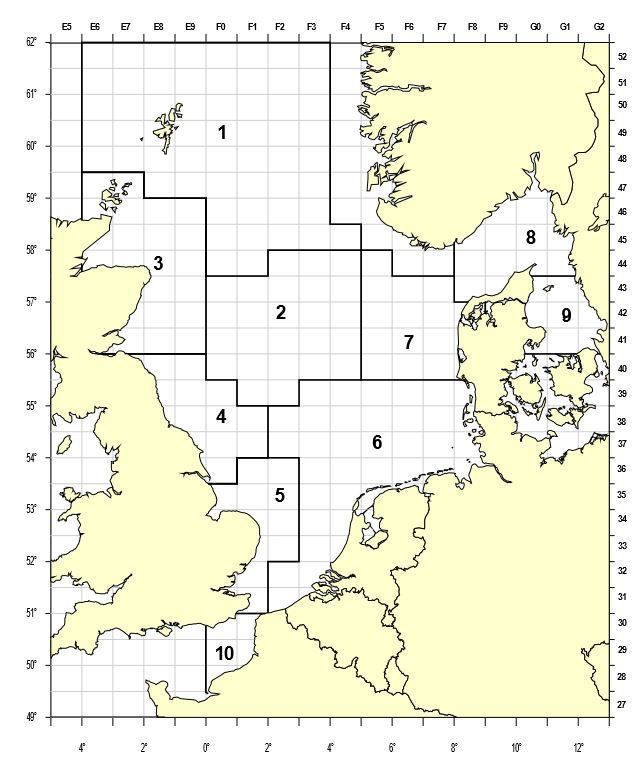
\includegraphics[width=17cm]{icesroundfishmap.jpg}}   
 \captionsetup{font= footnotesize, width=15cm}{
 \caption{Standard roundfish areas used for roundfish since 1980, for all standard species since 1991. Additional RFA 10 added in 2009. For example, the number 1 indicates ICES Index Area 1, and an ICES Statitical rectangle (ST) in IA 1 is 43F1.}\label{icesroufismap}}
\end{figure}

\clearpage

\section{Plots of Door Spread}
\begin{figure}[h!]
\begin{tabular}{ll}
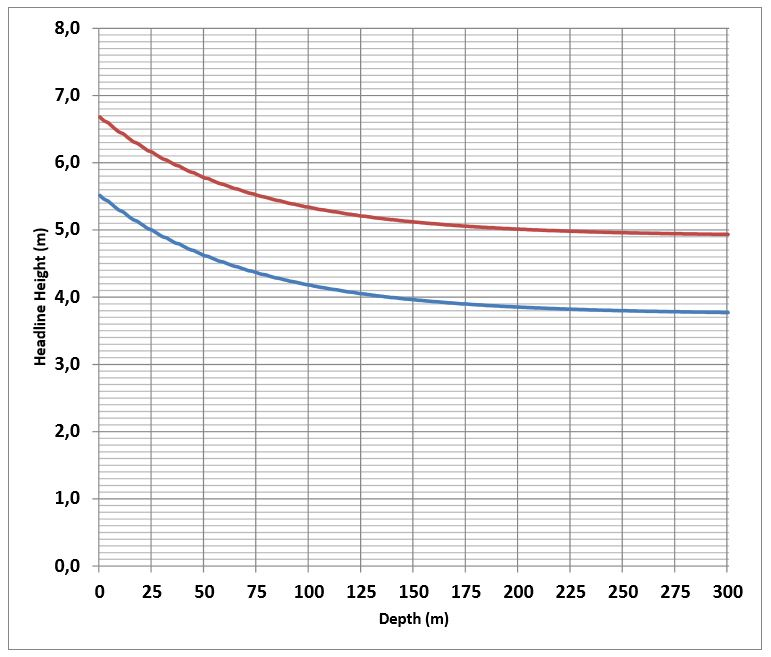
\includegraphics[scale=0.5]{headlineHeight.jpg}
&
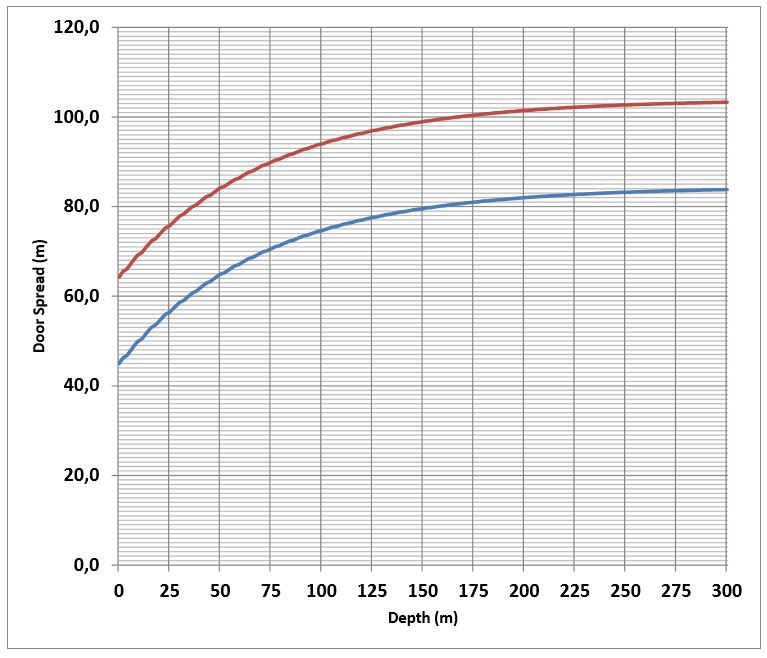
\includegraphics[scale=0.5]{doorspead.jpg}
\end{tabular}
\caption{Left: Expected upper and lower limits of Headline height for water %depth (ICES 2012). 
Right: Expected upper and lower limits of Door spread for water depth (ICES 2012).}
\label{fig:test}
\end{figure}

\clearpage

\section{Plots of Trawl Hauls with Age and Length }

\begin{figure}[h!]
  \centering
 {\includegraphics[width=17.5cm]{"Pollachius virens1".pdf}}   
 \captionsetup{font= footnotesize, width=15cm}{
 \caption{Plots of RFAs with trawl hauls having length and age information of Saithe in the first quarter of 2017. }\label{saithe}}
\end{figure}

%\clearpage
\begin{figure}[h!]
  \centering
 {\includegraphics[width=17.5cm]{"Gadus morhua1".pdf}}   
 \captionsetup{font= footnotesize, width=15cm}{
 \caption{Plots of RFAs with trawl hauls having length and age information of Cod in the first quarter of 2017. }\label{saithe}}
\end{figure}


%\end{appendices}


\clearpage

\bibliographystyle{apalike}
\bibliography{ibtsBib}
\end{document}